\documentclass[12pt,a4paper]{article}
\usepackage[utf8]{inputenc}
\usepackage[brazil]{babel}
\usepackage{enumitem}
\usepackage{graphicx}
\usepackage{setspace}
\usepackage{anysize}
\usepackage{pslatex} %fonte times new roman
\usepackage{titlesec}
\usepackage[a4paper,left=3cm,right=2cm,top=3cm]{geometry}
\onehalfspacing
%\usepackage[alf]{abntex2cite}
\usepackage{fancyhdr}
%\fancyhf{}
\fancyfoot{}
%\lhead{}
\rhead{\thepage}
\rfoot{}


%tirar cabeçalho
\fancypagestyle{nohead}{
    \fancyhead{}
    \fancyfoot{}
    %\lhead{\theauthor}
    \rhead{\thepage}
    \rfoot{}
    \renewcommand{\headrulewidth}{0pt}
}
%tirar page
\fancypagestyle{nopagenumber}{
    %\lhead{\theauthor}
    \rhead{}
    \rfoot{}
    \renewcommand{\headrulewidth}{0pt}
}

\usepackage[style=abnt]{biblatex}
\addbibresource{bibliografia.bib}        % Seus arquivos de
%\addbibresource{outroarquivo.bib}

%\usepackage{fontspec}
%\setmainfont[
%BoldFont=arialbd.ttf,
%ItalicFont=ariali.ttf,
%BoldItalicFont=arialbi.ttf
%]{arial.ttf}


\usepackage{tocloft}
\renewcommand{\cftfigfont}{Figura }

\renewcommand{\headrulewidth}{1pt}
\begin{document}
	
	%capa
     \pagestyle{empty}
\begin{titlepage}
	\begin{center}
		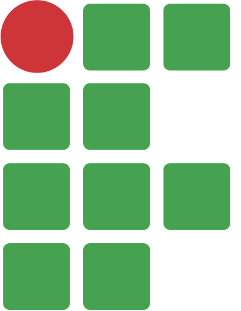
\includegraphics[width=2cm,height=3cm]{img/if}\\
		\textbf{INSTITUTO FEDERAL DE EDUCAÇÃO, CIÊNCIA E TECNOLOGIA DO CEARÁ IFCE CAMPUS ACARAÚ}
		\textbf{LICENCIATURA EM FÍSICA}\\
		\vspace{3cm}
		\textbf{MARCOS MAERLI PEREIRA}\\
		%Possivel titulo para TCC
				\vspace{4cm}
				\textbf{TEORIA DE RESPOSTA AO ITEM APLICADA A AVALIAÇÃO EDUCACIONAL}\\
				\vspace{6cm}
				\textbf{ACARAÚ - CE\\2017}
		\end{center}
	\end{titlepage}
\newpage
		\setcounter{page}{1}
		
	%folha de rosto
	   \begin{center}
		\textbf{MARCOS MAERLI PEREIRA}\\
		\vspace{6cm}
		\textbf{TEORIA DE RESPOSTA AO ITEM APLICADA A AVALIAÇÃO EDUCACIONAL}
		\vspace{2cm}
		\end{center}
		
            \newdimen\mylength
			\mylength = \linewidth
			\addtolength{\mylength}{-8.7cm}
						
			
			\hspace{8cm}\begin{minipage}{\mylength}
				
				Trabalho de Conclusão de Curso (TCC) apresentado ao curso de Licenciatura em Física do Instituto Federal
				de Educação, Ciência e Tecnologia do
				Ceará – IFCE – Campus Acaraú, como requisito
				parcial para obtenção do Título de Licenciado.
				\vspace*{0.7cm}
				\\Orientador (a): Prof. Dr hygor piaget monteiro melo
			\end{minipage}
			\par
			\vspace{7cm}
		\begin{center}
			ACARAÚ - CE\\
			2018
		\end{center}
		
	\newpage
	%folha de aprovação
	     \begin{center}
		\textbf{MARCOS MAERLI PEREIRA}\\
		\vspace{2cm}
		\textbf{TEORIA DE RESPOSTA AO ITEM APLICADA A AVALIAÇÃO ACADÊMICA}
	\end{center}
	\vspace{2cm}
		\hspace{\mylength}\begin{minipage}{8cm}
			
			Trabalho de Conclusão de Curso (TCC) apresentado ao curso de Licenciatura em Física do Instituto Federal
			de Educação, Ciência e Tecnologia do
			Ceará – IFCE – Campus Acaraú, como requisito
			parcial para obtenção do Título de Licenciado.
			\vspace*{0.7cm}
			\\Orientador (a): Prof. Dr hygor piaget monteiro melo
		\end{minipage}
		\par
	 \vspace{1cm}
	    Aprovada em \_\_/\_\_/\_\_\_\_\\
	    \vspace{1cm}
	\begin{center} 
	   
	    \textbf{BANCA EXAMINADORA} \\
	    \vspace{1.5cm}
    	\hrulefill\\
    	Prof. titulação - nome completo (Orientador (a))
    	instituição\\
    	\vspace{1.5cm}
    	\hrulefill\\
    	Prof. titulação nome completo (Orientador (a))
    	instituição \\
    	\vspace{1.5cm}
    	\hrulefill\\
    	Prof. titulação nome completo (Orientador (a))
    	instituição
    \end{center}
    \newpage

	%dedicatoria
	\begin{center}
	    \textbf{DEDICATÓRIA}
	\end{center}
	
	\newpage
	%AGRADECIMENTOS
	    \begin{center}
	    \textbf{AGRADECIMENTOS}
	\end{center}
	\par
        A Deus por tudo;
    \par
        Aos meus familiares e amigos;
    \par
        Agradeço aos professores que fizeram parte dessa jornada de busca do conhecimento aos professores Diego Sousa, Manoel Paiva, João Cláudio, Pablo Morais, Alessandro melo, Henrique camelo, João Neto, Loester Sá, Emanuel Viana, Avelar Macedo, Alex Samyr, Clerton, em especial ao professor George Frederick e Hygor Piaget, as Professoras Elizabeth Araújo, Marlene, Kiara Lima, Socorro Abreu, Alisandra, Sinara Rocha, Rosilane Costa;
    \par
        A CAPES pelo apoio institucional e finaceiro;
    \par
        Ao IFCE.
	\newpage
	\thispagestyle{empty}
	%resumo
	    \begin{center}
	    \textbf{RESUMO}
	\end{center}
	
	Desde os primórdios da sociedade humana moderna tem-se buscado avaliar as atividades humanas e suas respectivas habilidades, entretanto a forma que esta avaliação se dava era muito subjetiva, até que em meados do século 20, especialistas como matemáticos e psicomotristas criaram metologias capazes de medir grandezas próprias da natureza humana como habilidade ou proficiência em uma determinada área do conhecimento, com a criação da TCT evolui-se na medida de traços latentes, porém esta teoria tinha algumas limitações, a TRI veio para suprir estas carências, criando assim uma teoria capaz de medir com mais precisão os traços latentes, a TRI tem como característica básica a calibragem dos itens,ou seja a obtenção por meio de testes de três parâmetros: dificuldade, discriminação e acerto ao acaso. Devido a adoção o Enem da TRI,2009, no Brasil a TRI ganhou mais destaque, entretanto a complexidade matemática tem desencorajado professores na adoção desta metodologia para o uso em suas avaliações.
	\par
	\noindent Palavras Chaves: TRI, ENEM, teoria da medida.
	\newpage
	    
	%abstract
	           \begin{center}
	    \textbf{ABSTRACT}
	     \end{center}
	    \paragraph{}
	        In the beginning of modern human history, we are concerned how to evaluate the human tasks, and his corresponding abilities too. But, this kind of evaluation its depends on subject. Since the middle 20Th century, mathematicians and psicometrists created methodologies enabled to measure latent traits, such ability and proficiency in a specific area of knowledge. Since the CTT(Classical Test Theory) has been created a great evolution on the measurement theory. But CTT had some limitations, so IRT(Item Response Theory) comes to supply some of these limitations, this way was created a theory that measure with accuracy latent traits. It is IRT characterized by the item estimation  where testing we seek for three basic parameters: difficult, discrimination and casual percentage of correct answer. Due the adoption by Enem(An exam to measure ability of Brazilian high school students) from IRT, its has
	       been guarantee more visibility to the IRT in Brazil. But the math complexity has been discouraged teachers to apply IRT in his evaluations.
    \par
    keywords: IRT, Enem, Measurement theory.
	
	\newpage
	%\thispagestyle{nopagenumber}
	\renewcommand{\listfigurename}{\hfill LISTA DE ILUSTRAÇÕES\hfill}
	\listoffigures

	\newpage
	\thispagestyle{empty}
	\renewcommand{\contentsname}{\hspace{0.4\linewidth}SUMÁRIO}
	\tableofcontents
    
    \newpage
    
    \pagestyle{fancy}
	%introducao
	    \section{INTRODUÇÃO}
	\paragraph{}
	    \cite{MOREIRAJUNIOR} No início da colonização Brasileira, com a chegada dos portugueses juntamente com a (\textcite{OLIVEIRA}) Igreja Católica e também com a chegada da Ordem dos Jesuítas no ano de 1549. Os Jesuítas que acompanharam as grandes navegações, que tiveram atuação no Brasil de 1549 a 1759, estes tinham o objetivo de ensinar, catequizar e evangelizar a população nativa e para verificar os resultados de seus trabalhos aplicavam uma espécie de avaliação informal, chamadas provas orais, isto é, com o objetivo de analisar os ensinamentos dados a esta população de nativos sobre o Deus católico e a submissão à coroa portuguesa, verificar a aculturação e a conversão dos nativos, estes eram avaliados a partir da exposição de seus pensamentos pela oralidade, e escrita, em algumas situações. sendo esta uma forma de avaliação que apesar de válido, mostra-se totalmente dependente dos envolvidos.
	\paragraph{}
    	Nas décadas de 30 e 40, a partir da organização do Manifesto dos Pioneiros da Escola Nova, o processo de ensino e de aprendizagem é marca pela visão humanista do homem em relação ao homem tradicional, ou seja, há um equilíbrio no que diz respeito a concepção de homem, porém esse período não teve mudanças com importância significativa no que diz respeito ao modo de avaliar o aprendizado dos estudantes. Avaliar é parte fundamental do aspecto humano. todos nós somos avaliados de uma forma ou de outra, de forma voluntária quando postamos conteúdos nas redes sociais e o número de curtidas indicaram a aceitação do mesmo perante os amigos. Estes eventos ocorrem também no mundo acadêmico professores,alunos e instituições são avaliadas. Alunos são avaliados pelos professores a fim de verificarem a aprendizagem dos mesmos. Professores são avaliados a fim de avaliar o progresso diante do conteúdo a ser ministrado. As instituições são avaliadas por instâncias superiores como o MEC(Ministério da Educação). Todo este processo nos levar a acreditar que métodos  que tornem avaliações mais precisas devem ser implementados a TRI tem esse objetivo e o cumpre em partes. Daí no âmbito da educação avaliar faz parte de todo o processo de ensino. Segundo as leis brasileiras a avaliação tem esse fim.
	\par
	    \textcite{LDB} O Art. 9º, inciso VI da Lei de Diretrizes e Bases da Educação (LEI Nº 9.394, DE 20 DE DEZEMBRO DE 1996) versa sobre o objetivo da avaliação escolar, cabendo a União
		"VI - Assegurar processo nacional de avaliação do rendimento escolar no ensino fundamental, médio e superior, em colaboração com os sistemas de ensino, objetivando a definição de prioridades e a melhoria da qualidade do ensino."(BRASIl,1996,pag. 27833)
	\par
	    O processo avaliativo visa a melhoria e qualidade do ensino, então instrumentos que possibilitem uma melhor checagem dos dados também faz-se necessário.Por isso a TRI, supre essa carência de fala de instrumentos. 
	\par
	    Mediante as concepções que os alguns autores têm sobre avaliação podemos estabelecer critérios para avaliar, segundo Luckesi, "a avaliação é uma apreciação qualitativa sobre dados relevantes do processo de ensino e aprendizagem que auxilia o professor a tomar decisões sobre o seu trabalho.” Isso sugere que os dados quantitativos não são suficientes para avaliar há a necessidade que a avaliação seja também qualitativa, por tanto os instrumentos de medida devem prover os dados quantitativos e também uma forma de avaliar qualitativamente. Ainda segundo Luckesi (1978) a avaliação é definida como um julgamento de valor sobre manifestações relevantes da realidade, tendo em vista uma tomada de decisão.
	\par
	    Diante deste ponto de vista sobre avaliação. destaca-se os três principais tipos de avaliação.
	\subsection{TIPOS DE AVALIAÇÃO}
	\paragraph{}
	\subsection{avaliação diagnóstica}
	\paragraph{}
	    Tem como pressuposto básico detectar ou fazer uma verificação dos conteúdos e conhecimento do aluno. E a partir dos dados desse diagnóstico realizar o planejamento de ações que supram as necessidades e atinja os objetivos propostos. Com isso se utiliza a avaliação de aprendizagem como suporte para o planejamento de ensino. Sendo este tipo de avaliação aplicado no início do processo de ensino-aprendizagem.
	\subsection{avaliação formativa}
	\paragraph{}
	    Tem o objetivo verificar se o conteúdo proposto pelo professor no seu planejamento em relação aos conteúdos estão sendo atingidos durante todo o processo de ensino aprendizagem do aluno passo a passo. Com isso é possível aplicar a recuperação paralela, onde os alunos resgatam os conceitos revisando-os ao longo do caminho e evoluindo cada um no seu ritmo.
	\par
	    Essa intervenção e postura do professor como mediador tira de cena aquela prática de classificar o aluno com uma nota. Não se tem mais a visão da avaliação no resultado do teste e sim no potencial de desenvolvimento do aluno. O professor como mediador refletirá sobre o processo e tomar decisões para re-planejar suas ações para intervir e adequar suas práticas em sala de aula com o objetivo do aluno aprender e não simplesmente melhorar sua nota.
	\subsection{avaliação somativa}
	\paragraph{}
	    Tipo de avaliação que ocorre ao final da instrução com a finalidade de verificar o que o aluno efetivamente aprendeu. Inclui conteúdos mais relevantes e os objetivos mais amplos do período de instrução; visa à atribuição de notas; fornece \textit{feedback} ao aluno (informa-o quanto ao nível de aprendizagem alcançado), se este for o objetivo central da avaliação formativa; e presta-se à comparação de resultados obtidos com diferentes alunos, métodos e materiais de ensino. Foi assim classificada por Benjamin Bloom e seus colaboradores, cujos estudos apontam para outros dois tipos de avaliação: a formativa e a diagnóstica.\textcite{Takuno}
	\par
	    Tem o objetivo de atribuir notas e conceitos para o aluno ser promovido ou não de uma classe para outra, ou de um curso para outro, normalmente realizada durante o bimestre ou semestre.
		Segundo Luckesi, O professor deve aprender a avaliar, os professores devem aprender a avaliar, ou seja, professores são parte do processo avaliativo.
	    A TRI pode ser aplicada a cada uma destes três principais formas de avaliação.
	
	
	\newpage
	
	%secao  - teoria de resposta ao item
	    \section{TEORIA DE RESPOSTA AO ITEM}
	\subsection{Introdução}
	\paragraph{}
	    A busca por informações de medidas de propriedades psicológicas dos indivíduos levou muitos pesquisadores a desenvolver modelos que pudessem estimar essas tais propriedades psicológicas, também referidas por traço latente, que são características individuais que não podem ser observadas diretamente, como por exemplo habilidade/proficiência em determinado conteúdo na avaliação educacional, atitude em relação à mudança organizacional, nível de ansiedade, nível de estresse, nível de depressão, qualidade de vida etc.).\textcite{Araujo}
	\par
		De acordo com \textcite{Dalton}, a Teoria da Resposta ao Item (TRI) é uma metodologia que sugere formas de representar a relação entre a probabilidade de um indivíduo dar uma resposta correta a um item, ver figura(\ref{fig:ques}) e seus traços latentes. Entretanto a TRI teve seus primórdios com a Teoria Clássica dos Testes(TCT). O presente trabalho não aborda todas os modelos da TRI e não busca esgotar o tema, pois trata-se de um tema muito complexo, teórico-matematicamente, e tem por objetivo mostrar a sua viabilidade para pesquisadores e seu uso mais difundido.
	\par
		Os teste e questionários são os principais agentes responsáveis pela coleta de informações, assim cabe distinguir o que é um item, ver figura(\ref{fig:ques}). Sendo que teste é um instrumento ou uma ferramenta usada para fazer determinada medição(\cite{James}), sendo composto por diversos itens. Neste trabalho trata-se item e questão como sinônimos.
	\begin{figure}[!h]
		\centering
		\caption{Estrutura de um item}
		\fbox{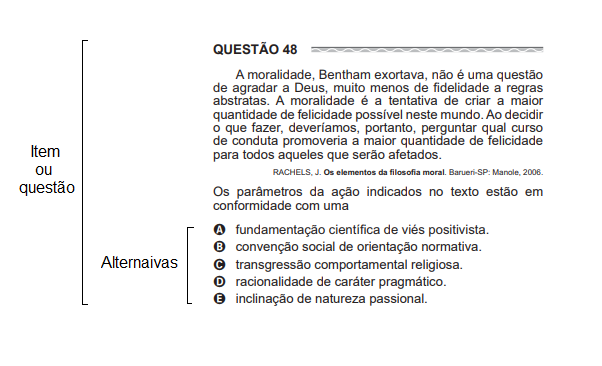
\includegraphics[width=0.5\linewidth]{img/ques.PNG}}\\
		Fonte: Questão 48 Enem 2017 / Primeiro Dia / Caderno azul .
		\label{fig:ques}
	\end{figure}
	\par
	    Assim o item é todo o conjunto: comando e as alternativas, sendo que uma das alternativas é a correta as as outras são apenas distratores, por isso diz-se itens dicotômicos(certo/errado). Quando um indivíduo endossa o item/questão diz-se que este acertou o item.
	 \par
		Um teste de múltipla consiste na escolha N itens ou questões, em geral, com 4 ou 5 alternativas de respostas, sendo uma, e somente uma, correta. O resultado é dado pelo número de acertos ou pelo percentual de acertos em uma escala própria de 0(zero) a 100 (cem), tomando como base a TCC(Teoria Clássica dos Testes). Em geral, não há julgamento sobre o que uma determinada nota significa, a não ser que notas acima de 70 costumam ser consideradas adequadas.\cite{Klein}
	
	\subsection{Teoria Clássica dos Testes(TCT)}
	\paragraph{}
	    Considerando um teste e seu escore Frederic Lord fez uma importante observação que o escore observado e o score verdadeiro de indivíduos examinados não tem o mesmo significado que a habilidade do indivíduo. Indivíduos podem ter baixos escores verdadeiros em um teste difícil e altos escores verdadeiros em um teste fácil, porém sua habilidade se mantém constante em relação qualquer outro teste que faça medição deste constructo. Claro que está habilidade esta sujeita à mudanças ao longo do tempo devido ao aprendizado posterior, porém no momento da aplicação do teste esta habilidade se mantém constante.
	\par
	    Lord e outros psicomotristas estavam interessados em um modelo que fossem independentes do conjunto de itens de um teste, No pensamento de Charles Spearman \cite{Spearman}, um dos fundadores da Teoria Clássica dos Testes, existiam erros nas medidas e que  erros eram variáveis aleatórias e que eles podiam ser correlacionados e classificados.
	\par
		Os testes de inteligência nas 4 primeiras décadas do seculo 20 levaram a criação da TCT\cite{Klein} muitos dos termos utilizados como score verdadeiro foi criada por Spearman's na sua teoria da inteligencia.
	\par
	    Segundo \textcite{Hamblenton} a TCT assume que cada pessoa tem um score verdadeiro, quando não há erros relacionados, o escore esperado para uma pessoa é dado por:
	 \par
	    \begin{equation}
	       X = T + E
	    \end{equation}
	\paragraph{}
	    Sendo que escore individual é o total de pontos em testes\cite{Ribeiro}.E $T$ o escore verdadeiro, $X$ o escore observado $X$ é o escore obtido por um estudante em um teste. E $E$ o erro relacionado.
	\par
	    Para cada indivíduo  existem duas incógnitas nesta equação, a é equação não pode ser resolvida a menos que algumas suposições sejam feitas.\cite{Klein}
	\paragraph{}
	\begin{enumerate}[label={\alph*)},noitemsep]
        \item escores verdadeiros e erro score são não correlacionados.
        \item a média do escore de erro na população de examinados é zero.
        \item o erro de score em testes paralelos(ver testes paralelos) são não correlacionados.
	\end{enumerate}
	\par
	   Por exemplo, Supondo que alguém saiba $70\%$ de um conteúdo este seria seu escore verdadeiro($T$), supondo existir um teste ideal ele mediria este escore, mas na realidade os testes medem um escore de $65\%$ a $75\%$ sendo que a discrepância de $5\%$ é o erro do escore.
	%$http://www.statisticshowto.com/classical-test-theory/$
    \par
    	No exemplo da tabela(\ref{tab:pessoas1}) exemplo, Pessoa 1 que respondeu todas as 5 itens corretamente, possui uma proficiência de $100\%$. \cite{Chong}. Entretanto não podemos julgar a proficiência de um indivíduo apenas com base no número de itens que este indivíduo acertou.
    \paragraph{}
    \begin{table}[!h]
    	\centering
    	\caption{Respostas de 5 pessoas a um teste hipotético}
    	\begin{tabular}{*{6}{c|}c}
    	    \hline
    	    resp & item 1& item 2& item 3 & item 4 & item 5 & score observado($X$)\\
    	    \hline
    	    \hline
    	     Pessoa 1 &  1 & 1 & 1 & 1 & 1 & 1\\
    	     Pessoa 2 &  1 & 1 & 1 & 1 & 0 & 0.8\\
    	     Pessoa 3 &  1 & 1 & 1 & 0 & 0 & 0.6\\
    	     Pessoa 4 &  1 & 1 & 0 & 0 & 0 & 0.4\\
             Pessoa 5 &  1 & 0 & 0 & 0 & 0 & 0.2\\
             Média &     1 & 0.8 & 0.6 & 0.3 & 0.2\\
             \hline
    	\end{tabular}
	    \label{tab:pessoas1}
	\end{table}
	\paragraph{}
		No exemplo da tabela(\ref{tab:pessoas2})em que a Pessoa 4 e a pessoa 6 tiveram o mesmo score, porém responderam itens diferentes, apesar de terem mesmo score não podemos afirmar nada sobre a proficiência de ambos os respondentes pois a pessoa 4 pode ter acertado itens fáceis enquanto a pessoa 6 acertado itens difíceis.
    \paragraph{}
	\begin{table}[!h]
	    \centering
	    \begin{tabular}{*{6}{c|}c}
	    \hline
	    respondente & item 1& item 2& item 3 & item 4 & item 5 & score observado($X$)\\
	    \hline
	    \hline
	        Pessoa 4 &  1 & 1 & 0 & 0 & 0 & 2\\
            Pessoa 5 &  1 & 0 & 0 & 0 & 0 & 1\\
            Pessoa 6 &  0 & 0 & 0 & 1 & 1 & 2 \\
            \hline
	    \end{tabular}
	    \caption{Respostas de 3 pessoas a um teste hipotético}
	    \label{tab:pessoas2}
	\end{table}
	\paragraph{}
		O quadro(\ref{tab:comparacao}) mostra as principais diferenças entre a TCT e a nova teoria que surgiria(TRI). E a TCT tinha também algumas limitações:
	\paragraph{}
    	\begin{enumerate}[noitemsep]
    	    \item As estatísticas que descrevem os itens de teste dependem do grupo de estudantes que fazem o teste.\\
            \item Os escores de teste que descrevem o desempenho dos alunos dependem dos itens apresentados aos alunos\\
            \item A Teoria Clássica dos Testes só pode ser utilizada em situações nas quais todos os alunos fazem o mesmo teste (ou formas “paralelas” de teste).\\
            \item A Teoria Clássica dos Testes não fornece um modelo do desempenho de um aluno em um item\\
            \item A maioria das aplicações da Teoria Clássica dos Testes assume incorretamente que os erros de medida têm a mesma variabilidade para todos os alunos. (Alguns aspectos da Teoria de Resposta ao Item relativos à estimação das proficiências)
	    \end{enumerate}
	\paragraph{}
	    Segundo \cite{Ronald} estas são as principais comparações entre TRI e TCT.
	\begin{table}[!h]
	    \centering
	    \caption{Comparação entre TCC e TRi}
	    \begin{tabular}{|p{4cm}|p{4cm}|p{4cm}|}
	        \hline
	         Área & TCT & TRI \\
	         \hline
	         \hline
	         Modelo & Linear & não-linear\\
	         \hline
	         Nível & Teste & Item \\
	         \hline
	         Habilidade item relação & Não especificado & CCI(curva caracteristica do item)\\
	         \hline
	         Invariancia entre item e a estatistica pessoal & Test scores or esti mated true scores are reported on the test-score scale (or a transformed test-score scale) & Ability scores are reported on the scale -00 to +00 (or a transformed scale)\\
	         \hline
	         Item statistics & p, r & b, a, and c (for the three-parameter model) plus corresponding item information functions \\
	         \hline
	         Sample size (for item parameter estimation) & 200 to 500 (in general) & Depends on the IRT model but larger samples, i.e., over 500, in general, are needed)\\
	         \hline
	    \end{tabular}
	     \label{tab:comparacao}
	\end{table}
	  
	\paragraph{}
	    Neste contexto A TRI foi desenvolvida principalmente para suprir limitações que a Teoria Clássica de Medidas /Teoria Clássica dos Testes(TCT) apresentava. dentre as quais se destaca que o instrumento de medida é dependente das características dos examinados que se submetem ao teste ou ao questionário.
	\par
	    Na TCT, a habilidade é medida da seguinte forma, o score total é a soma do número de questões corretas, na tentativa de estabelecer um nível de dificuldade ao teste, atribui-se pesos aos itens que compõem este teste. porém o modelo da TCT não consegue prever a coerência pedagógica e o “chute”.
	\par
	    A TRI tem uma abordagem diferente da TCT, o foco não está no teste e tratamos de probabilidades de de um individuo endossar um item, não tratamos de score e sim de habilidades. Porém a TRI não substitui a TCT.
	%(http://www.usf.edu.br/galeria/getImage/427/604207176923293.pdf)
		
	\newpage
	\subsection{Abordagem histórica}
	\paragraph{}
	    Segundo \textcite{Dalton} os primeiros modelos matemáticos que implementaram a TRI foram os dicotômicos, cujos possíveis resultados eram certo/errado ou concordo/descordo e outras variações de mesma natureza. Seja a resposta a um item $U_{ij} = 1$ para certo ou $U_{ij} = 0$ para item errado. Então surge a necessidade de encontrar uma função não linear que expressasse a probabilidade do respondente em função de sua habilidade dar uma resposta correta em função dos parâmetros do item. A própria necessidade desta função já impunha a restrição da CCI ser monótona crescente. %$https://www.maxwell.vrac.puc-rio.br/5253/5253\_4.PDF$
    \par	 
        Motivado pelo trabalho de \textcite{Lord}, Birnbaum fez uma modificação importante na teoria defendida por Lord, sugeriu a troca da função ogiva normal, proposta por Lord, pelo modelo logístico de dois parâmetros, por questões de conveniência. Além disso, foi Birnbaum, também, quem introduziu o terceiro parâmetro (vulgarmente conhecido como parâmetro de acerto casual, que modela um acerto em um teste educacional devido a um chute na questão)
	\par
		Como já foi dito, a TRI teve seus axiomas elaborados aos poucos desde os anos 50 por vários autores, embora suas raízes remontem há mais de uma década anterior. Entre estes precursores se encontram os trabalhos de Richardson (1936), comparando os parâmetros dos itens obtidos pela teoria clássica da Psicometria com os moldes que hoje usa a TRI. os trabalhos de Lawley (1943, 1944).
		Entretanto, o responsável mais direto que deu origem à TRI moderna, é Frederic Lord (1952, 1953).
		%http://pepsic.bvsalud.org/pdf/avp/v2n2/v2n2a02.pdf
	\par
        \textcite{Lord} foi o primeiro a desenvolver o modelo unidimensional de 2 parâmetros, baseado na distribuição normal. Após algumas aplicações desse modelo, o próprio Lord sentiu a necessidade da incorporação de um parâmetro que tratasse do problema do acerto casual. Assim, surgiu o modelo de 3 parâmetros. Anos mais tarde, \textcite{Birnbaum} substituiu, em ambos os modelos, a função ogiva normal pela função logística, matematicamente mais conveniente, pois é uma função explícita dos parâmetros do item e de habilidade e não envolve integração. Independentemente do trabalho de Lord, Rasch (1960) propôs o modelo unidimensional de 1 parâmetro, expresso também como modelo de ogiva normal e, também mais tarde descrito por um modelo logístico por Wright (1968).
        %teste
        \cite{Hamblenton}
	\subsection{Modelagem estatística da TRI}
	\paragraph{}
    	A TRI(Teoria de Resposta ao Item) é um conjunto de modelos estatísticos-matemáticos que procuram representar a probabilidade de um indivíduo dar uma resposta correta a um item como função dos parâmetros deste item e da habilidade (ou habilidades) do respondente. Essa relação é sempre expressa de tal forma que quanto maior a habilidade, maior a probabilidade de acerto no item, figura(). Segundo \textcite{Dalton}, os vários modelos propostos na literatura dependem fundamentalmente de três fatores:\\
    	\begin{enumerate}
    	    \item da natureza do item | dicotômicos(Figura 1) ou politômicos(Figura 2);
    	    \item do número de populações envolvidas | apenas uma ou mais de uma;
    	    \item da quantidade de traços latentes que está sendo medida | apenas um(modelo unidimensional) ou mais de um.
    	\end{enumerate}
    \paragraph{}
    	Entende-se por natureza dicotômica itens que aceitem certo/errado ou concordo/descordo como possíveis respostas, e itens politômicos sendo itens que contenham mais de três opções de respostas certo/errado/meio certo pu nenhum pouco/só um pouco/bastante/demais. Uma questão politômica pode ser observada no questionário  SNAP, questionário  para levantamento de alguns  possíveis  sintomas  primários  do  TDAH, como pode ser observado neste item:
    \newpage
	\begin{enumerate}
	    \item[H1] Não consegue prestar muita atenção a detalhes ou comete erros por descuido nos trabalhos da escola ou tarefas.
	    \begin{enumerate}
	        \item nenhum pouco
	        \item só um pouco
	        \item bastante
	        \item demias
	    \end{enumerate}
	\end{enumerate}
\par
	    A escolha da população fica a critério do pesquisador/avaliador, exemplo: podemos numa escola que tenham duas turmas de 5º ano, uma diurna outra noturna podemos fazer a escolha da população considerando apenas o 5º ano como uma população ou duas populações 5º ano A e 5º ano B. %O Enem utiliza
	\par
    	Explicam que o modelo de Rasch tem como uma de suas características fundamentais a premissa de que o comportamento de um. sujeito frente a um item pode ser explicado em função das características ou das atitudes
    	latentes $(\theta)$, que não são observadas diretamente. Nesse sentido, a variável latente de um
    	sujeito, o traço, influi sobre a probabilidade de acertar um item específico.
	 \par
	 	Quanto a quantidade de traços latentes trata-se do conceito muito importante para a escolha de qual modelo implementar. Quando estamos interessado em medir apenas um traço latente temos que utilizar modelos unidimensionais, caso contrario buscamos os modelos multidimensionais.
	 \par 
	    Busca-se através do modelo da unidimensionalidade encontrar apenas uma habilidade responsável por todas as outras habilidades. Sabemos que as atividades humanas requerem múltiplas habilidades para que uma determinada tarefa seja executada,  para a habilidade ou proficiência de um indivíduo não é diferente, um item para ser respondido corretamente necessita de diversas habilidades. Então para que haja a unidimensionalidade é necessário supor que existe uma habilidade responsável pelas demais habilidades necessárias para o endosso ao item. Porém existem modelos que supõem que mais de uma habilidade está sendo medida, os chamados modelos multidimensionais.
	 \par
		Traços latentes são características do indivíduo que não podem ser medidas diretamente, ou seja, não existe um aparelho capaz de medi-las diretamente, como nível de ansiedade, nível de depressão, proficiência, níveis de uma determinada emoção etc. Portanto, essas características são mensuradas através de variáveis secundárias que sejam relacionadas com o traço latente em estudo. Na busca por instrumentos que medissem traços latentes, a psicometria responsável pela junção da psicologia com as ciências exatas, apoderou-se de uma gama de modelos estatísticos que busquem estimadores para do parâmetro a ser medido.
	\par
	    Um traço latente deve ser inferido a partir da observação de variáveis secundárias que estejam relacionadas a ela, ou seja, a resposta do indivíduo. As características ocultas são difíceis de serem quantizadas por se tratarem de quantidades subjetivas.\\ 
	\par
	    os traços latentes se diferem de outras medidas por não poderem ser medidas por instrumentos físicos, por exemplo a massa e a temperatura que podem ser medidas por uma balança e termômetro.
	\par
	    Assim, se um pesquisador deseja obter a medida de um determinado traço latente, ele deve caracterizar a natureza do traço latente a ser medido, construir os itens que devem cobrir todo o traço latente, observar o tipo de resposta que é dado ao item para verificar se os itens têm natureza acumulativa ou de desdobramento e, a partir daí, escolher o modelo da TRI mais adequado que se ajuste ao seus dados. Em seguida, estimar os parâmetros dos itens e dos respondentes e construir e interpretar a escala do traço latente.
	\par
	    No âmbito da avaliação educacional a habilidade/proficiência de um aluno/respondente é o  traço latente no qual busca-se estimar. No entanto a função para o estimador da  habilidade de um respondente, não pode ser tida como uma função linear, ou seja, não é necessariamente verdade que a probabilidade de um aluno dar uma resposta correta a um item seja diretamente proporcional a sua habilidade. Por isso  A TRI(Teoria de Resposta ao item) surge como um conjunto de modelos matemáticos  que teve seus princípios básicos estabelecidos nos anos 1960, tomando conta de grande parte da psicometria nos anos 1980. Estas teorias postulam que o comportamento humano é consequência de processos hipotéticos chamados de traços latentes. Assim indivíduos com baixa habilidade tem baixa probabilidade de acertar o item e indivíduos com alta habilidade tem alta probabilidade de acertar o item.O modelo expressa a relação entre os comportamentos que são as respostas dadas aos itens as chamadas variáveis observáveis e os traços latentes (as variáveis hipotéticas) através uma equação matemática chamada de equação logística. Esta produz uma curva ou ogiva conhecida como a curva característica do item, a CCI. A CCI define os parâmetros dos comportamentos, ditos itens (dificuldade, discriminação e acerto casual) em função do tamanho do traço latente, expresso como teta $\theta$.\cite{Pasquali}
	\par
    	Neste trabalho utiliza-se para referência ,modelos que envolvem uma única população, o modelo logístico de 3 parâmetros e o modelo dicotômico, assim o modelo matemático utilizado será: modelo logístico unidimensional de 3 parâmetros (ML3). Sendo que o ML1 e ML2 podem ser obtidos a partir do ML3.
    	
    	%http://georgek.people.uic.edu/Karabatsos.pdf
    	
    \newpage
    	\noindent Definição função logística para o estimador:\\
	\begin{equation}
		P_i(U_{ij} = 1,\theta_j) = c_i + (1-ci)\displaystyle\frac{1}{1 + e^{-Da_i(\theta_j - b_i)}}
	\end{equation}
	    Onde:\\
	\begin{enumerate}[noitemsep]
	    \item[]  $0 < P_i < 1$ é a probabilidade de um respondente j com uma habilidade $\theta$ responder corretamente um item i com dificuldade b.
	    \item[] O parâmetro $b_i$  representa a dificuldade do   item i.
	    \item[] O parâmetro $a_i$ representa a discriminação do item i.
	    \item[] O parâmetro $c_i$ representa a probabilidade de um a um respondente com baixa habilidade responder corretamente ao item,  também conhecido como parâmetro de “chute”.
	    \item[] $\theta_j$ representa  a habilidade do respondente j.
	    \item[] $e$ é a constante $2.7182...$, conhecido como Número de Euler.
    	\item[] $D$  é uma constante $1.7$ para se aproximar de uma curva de ogiva normal. 
	\end{enumerate}
	\paragraph{}
    	O parâmetro de dificuldade($b$) que está na mesma escala que a habilidade($\theta$) refere-se a habilidade miníma para um indivíduo responder corretamente a um item. Em outras palavras é o valor no qual $P(U_i = 1, \theta)  = 0.5$
    \par
	    O parâmetro de discriminação é a capacidade que um item tem de distinguir os indivíduos que têm a proficiência requisitada daqueles quem não a têm. É também um valor no qual a derivada de $P(U_i = 1, \theta )$  no ponto em que $b = \theta$, graficamente podemos ver na figura(\ref{fig:Rplo2}) que quanto maior o declive da curva para habilidades próximas a dificuldade do item podemos ter uma discrepância grandes nas probabilidades,ou seja, este  item discrimina quem sabe e quem não sabe.
	\paragraph{}
	\begin{figure}[!h]
	    \centering
	    \caption{Curva característica do item}
	    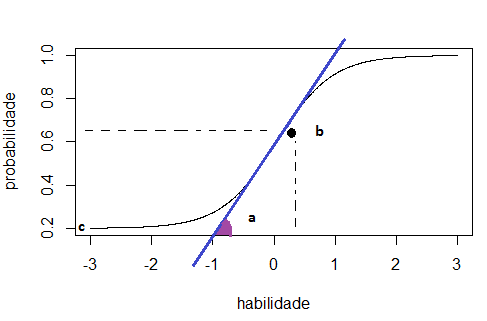
\includegraphics[width=0.48\linewidth]{img/Rplo2}\\
	    Fonte: Autor
	    \label{fig:Rplo2}
	\end{figure}
	\paragraph{}
    	\noindent A equivalência entre modelos ocorre quando:\\
    	O parâmetro de chute $c_i$ é igual a $0$ para todos os itens, que é equivalente ao modelo logístico de 2 parâmetros:
    \paragraph{}
	\begin{eqnarray}
		P_i(U_{ij} = 1,\theta_j) & = & c_i + (1-ci)\displaystyle\frac{1}{1 + e^{-Da_i(\theta_j - b_i)}} | c_i - 0 \nonumber \\ 
		P_i(U_{ij} = 1,\theta_j) & = & 0 + (1-0)\displaystyle\frac{1}{1 + e^{-Da_i(\theta_j - b_i)}} \nonumber \\
		P_i(U_{ij} = 1,\theta_j) & = & \displaystyle\frac{1}{1 + e^{-Da_i(\theta_j - b_i)}} \nonumber
	\end{eqnarray}
    	
    	\
    \noindent O parâmetro de chute é 0 e o parâmetro de discriminação é 1 sendo equivalente ao modelo logístico de 1 parâmetro\\
	
	\begin{eqnarray}
		P_i(U_{ij} = 1,\theta_j) & = & c_i + (1-ci)\displaystyle\frac{1}{1 + e^{-Da_i(\theta_j - b_i)}} | c_i - 0 | a_i = 1\\
		P_i(U_{ij} = 1,\theta_j) & = & 0 + (1-0)\displaystyle\frac{1}{1 + e^{-D*1*(\theta_j - b_i)}} \\
		P_i(U_{ij} = 1,\theta_j) & = & \displaystyle\frac{1}{1 + e^{-D*1*(\theta_j - b_i)}}
	\end{eqnarray}
    	
    \subsection{Modelo de Rasch}
    \paragraph{}
    	Rasch desenvolveu seu modelo independentemente da TRi, Sendo frequentemente considerado com o parametro de 1 parametro o modelo de Rasch apesar de alguns autores dierem ser uma bordagem totalmente diferente quanto aos conceitos.

	
\subsection{Curva característica do item}
    \paragraph{}
		Na definição moderna da TRI cada um dos itens terá uma curva característica(CCI), Segundo \cite{Baker}, Terman ainda na Teoria clássica dos testes, em 1916 Termam utilizando os dados das observações de Binet plotou a proporção de respostas corretas como função da idade cronológica na escala de inteligência de Binet-Simon, e traçou uma linha entre os pontos criando assim a CCI(\ref{fig:cci_age}). Binet colocou no teste de inteligencia um item cuja proporção de respostas corretas dadas pelos respondentes era de 0,75 , no caso da figura, mas qualquer outra proporção poderia ser usada, Termam utilizou a proporção 0,50. SendoTucker foi primeiro a utilizar a expressão curva característica do item.
	\begin{figure}[!h]
	    \centering
	    \caption{Plote de idade cronológica}
	    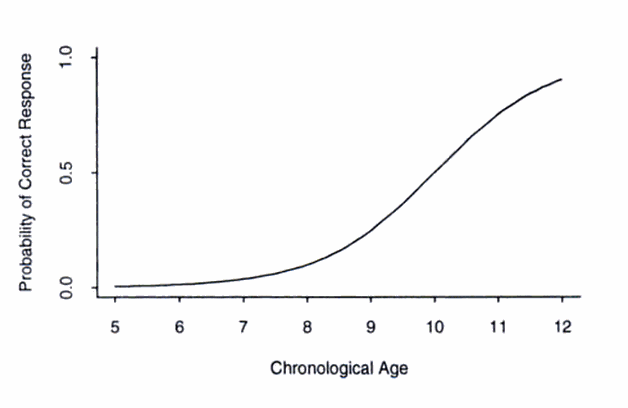
\includegraphics[width=0.5\linewidth]{img/age}
	    \label{fig:cci_age}
	\end{figure}
	   
	\paragraph{}
    	Assim podemos ver que a curva característica é a relação entre a proporção de respostas corretas ao item e uma variável de interesse, no caso de Binet a inteligência, na avaliação escolar a habilidade ou proficiência.
    \paragraph{}
    
    
    
        Os modelos dos modelos  curva características do item existentes, apenas dois são os mais utilizados: o modelo de ogiva normal e o modelo logístico normal. Muitas outras funções fora dessa classe foram propostas, tal como a função linear, mas com pouco efeito prático e sérias limitações nos valores possíveis para as habilidades(\cite{Ribeiro}).
    \subsubsection{Curva ogiva normal}
    \begin{figure}[!h]
    	\centering
    	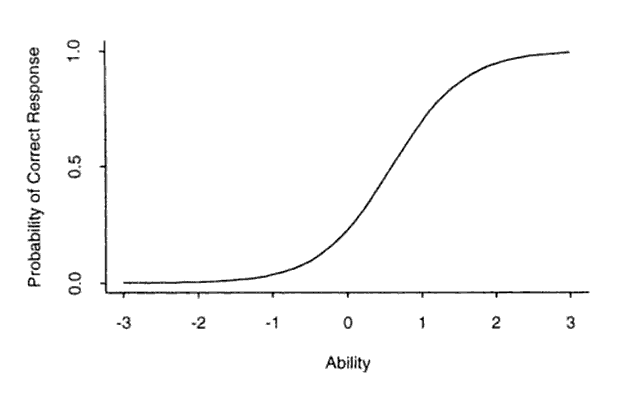
\includegraphics[width=0.6\linewidth]{img/ogiva}
    	\caption{}
    	\label{fig:ogiva}
    \end{figure}
    \paragraph{}
        Modelo proposto por Lord:
    \begin{equation}
        P(\theta) = \displaystyle\int_{-\infty}^{a_i(\theta - b_i)}\displaystyle\frac{1}{\sqrt{2\pi}}e^{-t^2/2}dt
    \end{equation}
    \paragraph{}
        Pode ser entendido de acordo com dois pontos de vista, Segundo (tem Response Theory: Parameter Estimation Techniques, Second Edition) autores como Richardson e Ferguson e Finney  simplesmente assumindo que a curva característica do item pode ser modelado por uma ogiva normal, fazendo teste e comparando as proporções de respostas corretas assim a ogiva normal provou-se se adaptar aos dados. a segunda explicação é dada por \cite{Novick} mais teórica.
        
    \subsubsection{Curva logística}
    \begin{figure}[!h]
    	\centering
    	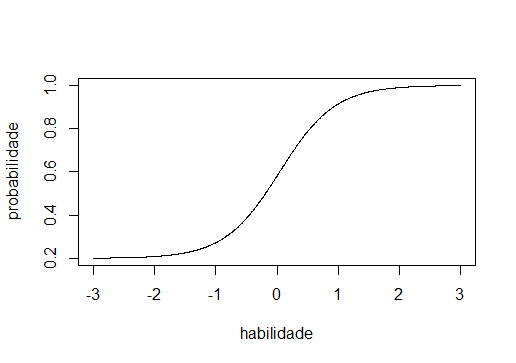
\includegraphics[width=0.6\linewidth]{img/Rplo}
    	\caption{}
    	\label{fig:rplo}
    \end{figure}
    \paragraph{}
        Muito similar ao modelo de ogiva normal, o segundo modelo, utilizado pela tri é o modelo logístico sendo atribuído a Birnbaum este modelo é também utilizado para o crescimento da população, plantas, pessoas. Segundo \cite{Baker} ambos modelos são usado em tri porem o modelo logístico é predominante na literatura acadêmica.
    \paragraph{}
        A forma da função logística:
    \begin{equation}
        P_i(\theta) = \displaystyle\frac{e^{Z_i}}{1 + e^{Z_i}} = \displaystyle\frac{1}{1 + e^{-Z_i}}
    \end{equation}
    
    Onde:\\
    $Z_i = a_i(\theta - b_i)$, também chamado de logit. 
    \paragraph{}
        O modelo de ogiva normal foi usado nos anos 1960, porem devido a demanda computacional que este modelo exigia foi preterido em relação ao modelo logístico. entretanto atualmente devido ao avanço dos computadores e com o de series polinomiais para funções de ogiva normal.
	\subsection{Conceitos Estatísticos}
    	Para melhor entendimento buscamos uma definição no livro \cite{Sonia}
	 \begin{enumerate}
	 	\item[]  \textbf{População} É uma coleção completa de todos os elementos a serem estudados.
	 	\item[] \textbf{Amostra} É uma subcoleção de elementos extraídos de uma população.
	 	\item[] \textbf{Parâmetro} É uma medida numérica que descreve uma característica de uma população.
	 	 \item[] \textbf{Estatística} É uma medida numérica que descreve uma característica de uma amostra.
	 	 \item[] \textbf{Estimador} É um regra para calcular uma estimativa de uma determinada quantidade baseada em dados observados.
	\end{enumerate}
	\paragraph{}
	    No âmbito da avaliação educacional a TRI  que procuram representar a probabilidade de um indivíduo dar uma certa resposta a um item como função dos parâmetros do item e da habilidade (ou habilidades) do respondente. Essa relação é sempre expressa de tal forma que quanto maior a habilidade, maior a probabilidade de acerto no item. Os vários modelos propostos na literatura dependem fundamentalmente de três fatores, está definição e da Tri voltada para a avaliação educacional.

	\newpage
	%secao - estimcao
	    \section{ESTIMAÇÃO}
	\paragraph{}
    	Existem vários casos que podem ser estimados. Sabe-se o parâmetros dos itens, e não as habilidades dos respondentes, 
    	Sabe-se as habilidades dos estudantes mas não sabe-se os parâmetros dos itens,e o caso mais comum quando não sabemos nem os parâmetros dos itens nem as habilidades dos respondentes, neste caso faz-se a estimação conjunta de parâmetros e habilidades.
	\par
	    Assim estimar os parâmetros dos itens tem como significado encontrar os valores dos parâmetros da função características do item que se ajustem aos dados, ou seja, encontrar os valores dos parâmetros a,b e c e $\theta$.
	\begin{figure}[!h]
	    \centering
	    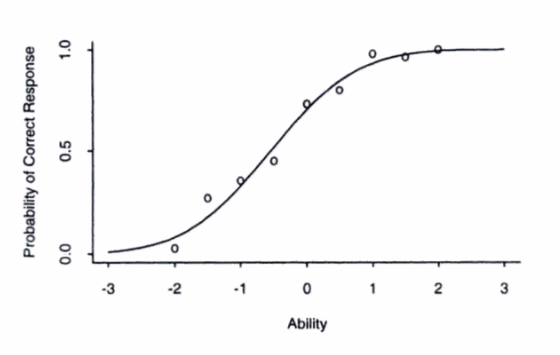
\includegraphics[width=0.6\linewidth]{img/proporcao}
	    \caption{Proporção de respostas corretas dada a um item}
	    \label{fig:proporcao}
	\end{figure}
	
	\subsection{Máxima-verossimilhança}
	\paragraph{}
	    O princípio de máxima verossimilhança(MVM) o procedimento usado para se obtenção de estimadores em estatística. Consideremos uma população e uma variável aleatória $X$, relacionada a essa população, com função de probabilidade (se é uma variável aleatória discreta) ou função densidade de probabilidade (se  é uma variável aleatória contínua) no nosso caso a função característica do item(CCI) , sendo  o parâmetro desconhecido. Retiremos uma amostra aleatória simples de , de tamanho $n$, e sejam  os valores efetivamente observados.\par
	    A função de verossimilhança  é definida por:
	\begin{equation}
	    L(\theta; x_1,x_2,...,x_n) = f(x_1;\theta) \times ... f(x_n;\theta) = \prod_{i = 1}^{n} f(x_i;\theta)
	    \label{fun:vero}
	\end{equation}
	    Onde $f(x_n;\theta)$ é a função de densidade de probabilidade, que deve ser interpretada como uma função de $ \theta $. O estimador de máxima verossimilhança de $ \theta $ é o valor que maximiza $ L(\theta;x_1,\ldots,x-n) $
	    Em muitos casos, o estimador de máxima verossimilhança pode ser encontrado seguindo os passos abaixo:\\
    \begin{enumerate}
        \item Encontrar a função de verossimilhança(\ref{fun:vero});
        \item Aplicar a função log;
        \item Derivar em relação ao parâmetro $ \theta , x_1,x_2...x_n$;
        \item Igualar o resultado a zero.
        \item Verificar que este estimador é ponto de máximo.
    \end{enumerate}
    \paragraph{}
	    Em outras palavras, tendo-se um conjunto de dados e um modelo estatístico, o método de máxima verossimilhança estima os valores dos diferentes parâmetros do modelo estatístico de maneira a maximizar a probabilidade dos dados observados (isto é, busca parâmetros que maximizem a função de verossimilhança). O método de máxima verossimilhança apresenta-se como um método geral para estimação de parâmetros, principalmente no caso de distribuições normais. Assim para encontrarmos o valor dos dados que maximizam a função de MV, precisamos derivar a função de MV e encontrar o valor que são raízes desta função derivada.
	\subsection{Estimação para uma única população}
	\cite{George} 
    	Considerando no caso de N indivíduos, $1 < j < N$, respondendo a I itens, $1 < i < I$, onde cada resposta é: $U_{ji} = 1$ como correta ou $U_{ji} = 0$ incorreta . Utilizando o MVM podemos estimar os parâmetros dos itens no modelo logístico de 3 parâmetros, temos as seguintes definições:
	\paragraph{}
	\begin{table}[!h]
	    \centering
    	\begin{tabular}{rl}
    	    $U_j = (U_{j1},U_{j2},...,U_{jI})$ & sendo o vetor de respostas do respondente j\\ 
        	$\zeta = (\zeta_1,\zeta_2,...,\zeta_I)$ & vetor de dos parâmetros dos itens\\
    	    $\theta = (\theta_1,\theta_2,...,\theta_N)$ & vetor de habilidades dos respondentes
    	\end{tabular}
	\end{table}
  
	$$
	U_{ij} = \left\{
	\begin{array}{ll}
    	1, resposta \quad correta,\\
    	0, resposta \quad incorreta.
    	
    	\end{array}\right.
	$$
	
	\subsubsection{Encontrando a função de verossimilhança}
	\paragraph{}
	    Para fazer a estimação dos parâmetros dos itens, temos que encontrar a função de máxima-verossimilhança, ver definição(\ref{fun:vero}), sendo o produto das probabilidades dos $N$ indivíduos responder corretamente o item $i$.
	\begin{eqnarray}
		L(\zeta) &=& \prod_{j = 1}^{n}P_i(U_{j.} = u_{j.}|\theta_j)\\
		L(\zeta) &=& \prod_{j=1}^{N}\prod_{i = i}^{I}P(U_{ij} = u_{ij}|\theta_j,\zeta_i)
	\end{eqnarray}
	
	\begin{eqnarray}
		P_{ji} &=& P(U_{ji} = 1|\theta_j,\zeta_i)\\
		Q_{ji} &=& 1 - P_{ji}
	\end{eqnarray}
	
	temos:
	
	\begin{eqnarray}
		P(U_{ji} = u_{ji}|\theta_j,\zeta_i) &=& P(U_{ji} = 1|\theta_j,\zeta_i)^{u_{ji}}P(U_{ji} = 0|\theta_j,\zeta_i)^{1 - u_{ji}}\\
		& = & P_{ji}^{u_{ji}}Q_{ji}^{1 - u_{ji}}
	\end{eqnarray}
	assim:
	
	$$
	L(\zeta) = \displaystyle\prod_{j = 1}^N\displaystyle\prod_{i = 1}^{I}P_{ji}^{u_{ji}}Q_{ji}^{1 - u_{ji}}
	$$
	
	\subsubsection{Aplicando a função log}
	\paragraph{}
	    Como devemos derivar a função de verossimilhança, derivar o produtorio de $N \times i$ termos é uma tarefa árdua, então podemos usar o artificio matemático de aplicar o logaritimo a $L(\zeta)$ visto que os mesmos parâmetros que maximizam a função $L(\zeta)$ são os mesmos para $\log(L(\zeta))$
	
	seguindo log-verossimilhança\\
	$$
	\log L(\zeta) = \displaystyle\sum_{j = 1}^{N}\displaystyle\sum_{i = 1}^{I}\{u_{ji}\log P_{ji} + (1 - u_{ji})\log Q_{ji}\}
	$$
	Os Estimadores de Máxima verossimilhança (EMV) de $\zeta_i$ , i = 1,..., I, são os valores que maximizam a verossimilhança, ou equivalente, são as soluções da equação:
	\subsubsection{Igualando a função igual a zero}
	$$
	\displaystyle\frac{\partial\log L(\zeta)}{\partial\zeta_i} = 0
	$$
	
	\begin{eqnarray}
		\displaystyle\frac{\partial\log L(\zeta)}{\partial\zeta_i} & = &\displaystyle\sum_{j = 1}^{N}\left\{u_{ji}\displaystyle\frac{\partial(\log P_{ji})}{\partial\zeta_i} + (1 - u_{ji})\displaystyle\frac{\partial(\log Q_{ji})}{\partial\zeta_i}\right\}\\
		& = & \displaystyle\sum_{j = 1}^{N}\left\{
		u_{ji}\displaystyle\frac{1}{P_{ji}}\left(\displaystyle\frac{\partial P_{ji}}{\partial \zeta_i}\right) - (1 - u_{ji})\displaystyle\frac{1}{Q_{ji}}\left(\displaystyle\frac{\partial P_{ji}}{\partial \zeta_i}\right)
		\right\}\\
		& = & \displaystyle\sum_{j = 1}^{N}\left\{u_{ji}\displaystyle\frac{1}{P_{ji}} - (1 - u_{ji})\displaystyle\frac{1}{Q_{ji}}\right\}\left(\displaystyle\frac{\partial P_{ji}}{\partial \zeta_i}\right)\\
		& = & \displaystyle\sum_{j = 1}^{N}
		\left\{
		\displaystyle\frac{u_{ji} - P_{ji}}{P_{ji}Q_{ji}}
		\right\}				
		\left(
		\displaystyle\frac{\partial P_{ji}}{\partial \zeta_i}
		\right)
	\end{eqnarray}
	
	por conveniência
	
	$$
	    W_{ji} = \displaystyle\frac{P_{ji}^{*}Q_{ji}^{*}}{P_{ji}Q_{ji}}
	$$
	
	onde,
	
	$$
	    P_{ji}^{*} = \{1 + e^{-Da_i(\theta_j - b_i)}\}^{-1} \quad  \mbox{e} \quad Q_{ji}^{*} = 1 - P_{ji}^{*}
	$$
	assim podemos escrever
	$$
	    \displaystyle\frac{\partial\log L(\zeta)}{\zeta_i} = \displaystyle\sum_{j = 1}^{N}
	    \left\{
	    (u_{ji} - P_{ji})\displaystyle\frac{W_{ji}}{P_{ji}^{*}Q_{ji}^{*}}			
	    \right\}
	    \left(
	    \displaystyle\frac{\partial P_{ji}}{\partial \zeta_i}
	    \right)
	$$
	para obter os parâmetros serão necessários:
	\begin{eqnarray}
		\displaystyle\frac{\partial P_{ji}}{\partial a_i} &=& D(1 - c_i)(\theta_j - b_i)P_{ji}^{*}Q_{ji}^{*}\\
		\displaystyle\frac{\partial P_{ji}}{\partial b_i} &=& -Da_i(1 -c_i)P_{ji}^{*}Q_{ji}^{*}\\
		\displaystyle\frac{\partial P_{ji}}{\partial c_i} &=& Q_{ji}^{*}
	\end{eqnarray}
	para o parâmetro de discriminação
	\begin{eqnarray}
		\displaystyle\frac{\partial \log(\zeta)}{\partial a_i} & = & \sum_{j = 1}^{N}\left\{
		(u_{ji} - P_{ji})\left(\displaystyle\frac{\partial P_{ji}}{\partial a_i}\right)\displaystyle\frac{W_{ji}}{P_{ji}^{*}Q_{ji}^{*}}
		\right\}\\
		&=& \sum_{j = 1}^{N}\left\{
		(u_{ji} - P_{ji})D(1 - c_i)(\theta_j - b_i)P_{ji}^{*}Q_{ji}^{*}\displaystyle\frac{W_{ji}}{P_{ji}^{*}Q_{ji}^{*}}
		\right\}\\
		& = & D(1 - c_i)\sum_{j = 1}^{N}(u_{ji} - P_{ji})(\theta_j - b_i)W_{ji}		
	\end{eqnarray}		
	
	parâmetro de dificuldade\\
	
	\begin{eqnarray}
		\displaystyle\frac{\partial \log(\zeta)}{\partial b_i} & = & \sum_{j = 1}^{N}\left\{
		(u_{ji} - P_{ji})\left(\displaystyle\frac{\partial P_{ji}}{\partial b_i}\right)\displaystyle\frac{W_{ji}}{P_{ji}^{*}Q_{ji}^{*}}
		\right\}\\
		&=& \sum_{j = 1}^{N}\left\{	
		(u_{ji} - P_{ji})(-1)Da_{i}(1 - c_i)P_{ji}^{*}Q_{ji}^{*}\displaystyle\frac{W_{ji}}{P_{ji}^{*}Q_{ji}^{*}}
		\right\}\\
		& = & -Da_{i}(1 - c_i)\sum_{j = 1}^{N}(u_{ji} - P_{ji})W_{ji}
	\end{eqnarray}		
	parâmetro acaso\\
	\begin{eqnarray}
		\displaystyle\frac{\partial \log(\zeta)}{\partial c_i} & = & \sum_{j = 1}^{N}\left\{
		(u_{ji} - P_{ji})\left(\displaystyle\frac{\partial P_{ji}}{\partial c_i}\right)\displaystyle\frac{W_{ji}}{P_{ji}^{*}Q_{ji}^{*}}
		\right\}\\
		&=& \sum_{j = 1}^{N}\left\{	
		(u_{ji} - P_{ji})Q_{ji}^{*}\displaystyle\frac{W_{ji}}{P_{ji}^{*}Q_{ji}^{*}}
		\right\}\\
		&=& \sum_{j = 1}^{N}\left\{	
		(u_{ji} - P_{ji})\displaystyle\frac{W_{ji}}{P_{ji}^{*}}
		\right\}\\
	\end{eqnarray}
	\subsubsection{Método de Newton-Raphson}
	\paragraph{}
        O Método de Newton-Rapshon na forma matricial verifica se o conjunto de parâmetros é ponto de máximo, Assim:\\
	    Seja $l(\zeta) = \log L(\zeta)$ a log-verossimilhança, onde $\zeta = (\zeta_1,\zeta_2,...,\zeta_I)$ com $\zeta_i = (a_i,b_i,c_i)$
	    os valores inicias são $\hat{\zeta}^{(0)} = (a_i^{(0)},b_i^{(0)},c_i^{(0)})$
	
    	a estimativa para $l(\zeta) = \log L(\zeta)$ será 
	    $\hat{\zeta}^{(1)} = \hat{\zeta}^{(0)} + \Delta\hat{\zeta}_i^{(0)}$
	    ou seja\\
	\begin{eqnarray}
		\hat{a}_i^{(1)} & = & \hat{a}_i^{(0)} + \Delta\hat{a}_i^{(0)}\\
		\hat{b}_i^{(1)} & = & \hat{b}_i^{(0)} + \Delta\hat{b}_i^{(0)}\\
		\hat{c}_i^{(1)} & = & \hat{c}_i^{(0)} + \Delta\hat{c}_i^{(0)}
	\end{eqnarray}
	Onde:\\
	
	$\Delta\hat{a}_i^{(0)}$,$\Delta\hat{b}_i^{(0)}$,$\Delta\hat{c}_i^{(0)}$ são os erros de aproximação.\\
	Usando a expansão de Taylor de $\displaystyle\frac{\partial l(\zeta)}{\partial \zeta_i}$\\
	\begin{eqnarray}
		\displaystyle\frac{\partial l(\zeta)}{\partial a_i} & = & \displaystyle\frac{\partial l(\hat{\zeta}_i^{(0)})}{\partial a_i} + \Delta\hat{a}_i^{(0)} \displaystyle\frac{\partial^2 l(\hat{\zeta}_i^{(0)})}{\partial a_i^2} + \Delta\hat{b}_i^{(0)} \displaystyle\frac{\partial^2 l(\hat{\zeta}_i^{(0)})}{\partial a_i \partial b_i} + 
		\Delta\hat{c}_i^{(0)} \displaystyle\frac{\partial^2 l(\hat{\zeta}_i^{(0)})}{\partial a_i \partial c_i} + R_{a_i}(\hat{\zeta}_i^{(0)}) \nonumber\\
		\displaystyle\frac{\partial l(\zeta)}{\partial b_i} & = & \displaystyle\frac{\partial l(\hat{\zeta}_i^{(0)})}{\partial b_i} + \Delta\hat{b}_i^{(0)} \displaystyle\frac{\partial^2 l(\hat{\zeta}_i^{(0)})}{\partial b_i^2} + \Delta\hat{b}_i^{(0)} \displaystyle\frac{\partial^2 l(\hat{\zeta}_i^{(0)})}{\partial b_i \partial a_i} + \Delta\hat{c}_i^{(0)} \displaystyle\frac{\partial^2 l(\hat{\zeta}_i^{(0)})}{\partial b_i \partial c_i} + R_{b_i}(\hat{\zeta}_i^{(0)}) \nonumber\\
		\displaystyle\frac{\partial l(\zeta)}{\partial c_i} & = & \displaystyle\frac{\partial l(\hat{\zeta}_i^{(0)})}{\partial c_i} + \Delta\hat{a}_i^{(0)} \displaystyle\frac{\partial^2 l(\hat{\zeta}_i^{(0)})}{\partial c_i^2} + \Delta\hat{b}_i^{(0)} \displaystyle\frac{\partial^2 l(\hat{\zeta}_i^{(0)})}{\partial c_i \partial a_i } + \Delta\hat{c}_i^{(0)} \displaystyle\frac{\partial^2 l(\hat{\zeta}_i^{(0)})}{\partial c_i \partial b_i}+ R_{c_i}(\hat{\zeta}_i^{(0)}) \nonumber
	\end{eqnarray}
	
	$$
	\displaystyle\frac{\partial l(\zeta_i)}{\partial a_i} = \displaystyle\frac{\partial l(\zeta_i)}{\partial b_i} = \displaystyle\frac{\partial l(\zeta_i)}{\partial c_i} = 0
	$$
	
	usando a notação \\
	
	\begin{eqnarray}
		L_1 = \displaystyle\frac{\partial l(\hat{\zeta}_i^{(0)})}{\partial a_i} \quad L_{11} =  \displaystyle\frac{\partial^2 l(\hat{\zeta}_i^{(0)})}{\partial a_i^2} \quad L_{12}  = \displaystyle\frac{\partial^2 l(\hat{\zeta}_i^{(0)})}{\partial a_i \partial b_i} \quad L_{13} = \displaystyle\frac{\partial^2 l(\hat{\zeta}_i^{(0)})}{\partial a_i \partial c_i} \nonumber\\
		L_2 = \displaystyle\frac{\partial l(\hat{\zeta}_i^{(0)})}{\partial b_i} \quad L_{21} = \displaystyle\frac{\partial^2 l(\hat{\zeta}_i^{(0)})}{\partial b_i^2} \quad L_{22} = \displaystyle\frac{\partial^2 l(\hat{\zeta}_i^{(0)})}{\partial b_i \partial a_i} \quad L_{23} =  \displaystyle\frac{\partial^2 l(\hat{\zeta}_i^{(0)})}{\partial b_i \partial c_i}\nonumber\\
		L_3 = \displaystyle\frac{\partial l(\hat{\zeta}_i^{(0)})}{\partial c_i} \quad L_{31} = \displaystyle\frac{\partial^2 l(\hat{\zeta}_i^{(0)})}{\partial c_i^2} \quad L_{32} = \displaystyle\frac{\partial^2 l(\hat{\zeta}_i^{(0)})}{\partial c_i \partial a_i } \quad L_{33} = \displaystyle\frac{\partial^2 l(\hat{\zeta}_i^{(0)})}{\partial c_i \partial b_i} \nonumber
	\end{eqnarray}
	Dezprezando os restos
	
	\begin{eqnarray}
		0 &=& L_1 + L_{11}\Delta\hat{a}_i^{(0)} + L_{12}\Delta\hat{b}_i^{(0)} + L_{13}\Delta\hat{c}_i^{(0)}\\
		0 &=& L_2 + L_{21}\Delta\hat{a}_i^{(0)} + L_{22}\Delta\hat{b}_i^{(0)} + L_{23}\Delta\hat{c}_i^{(0)}\\
		0 &=& L_3 + L_{31}\Delta\hat{a}_i^{(0)} + L_{32}\Delta\hat{b}_i^{(0)} + L_{33}\Delta\hat{c}_i^{(0)}
	\end{eqnarray}
	
	forma matricial
	
	$$
	-\left(\begin{array}{c}
	L_1\\
	L_2\\
	L_3\\
	\end{array}\right) =  
	\left(\begin{array}{ccc}
	L_{11} & L_{12} & L_{13}\\
	L_{21} & L_{22} & L{23}\\
	L_{31} & L_{32} & L_{33}\\
	\end{array}\right)
	\left(\begin{array}{c}
	\Delta\hat{a}_i^{(0)}\\
	\Delta\hat{b}_i^{(0)}\\
	\Delta\hat{c}_i^{(0)}\\
	\end{array}\right)
	$$
	
	Resolvendo o sistema para $\Delta\hat{\zeta}_i^{(0)}$, teremos
	
	$$		
	\left(\begin{array}{c}
	\Delta\hat{a}_i^{(0)}\\
	\Delta\hat{b}_i^{(0)}\\
	\Delta\hat{c}_i^{(0)}\\
	\end{array}\right) =  
	-\left(\begin{array}{ccc}
	L_{11} & L_{12} & L_{13}\\
	L_{21} & L_{22} & L{23}\\
	L_{31} & L_{32} & L_{33}\\
	\end{array}\right)^{-1}
	\left(\begin{array}{c}
	L_1\\
	L_2\\
	L_3\\
	\end{array}\right)
	$$
	
	assim\\
	$$		
	\left(\begin{array}{c}
	\hat{a}_i^{(1)}\\
	\hat{b}_i^{(1)}\\
	\hat{c}_i^{(1)}\\
	\end{array}\right) = 	
	\left(\begin{array}{c}
	\hat{a}_i^{(0)}\\
	\hat{b}_i^{(0)}\\
	\hat{c}_i^{(0)}\\
	\end{array}\right) 
	-\left(\begin{array}{ccc}
	L_{11} & L_{12} & L_{13}\\
	L_{21} & L_{22} & L{23}\\
	L_{31} & L_{32} & L_{33}\\
	\end{array}\right)^{-1}
	\left(\begin{array}{c}
	L_1\\
	L_2\\
	L_3\\
	\end{array}\right)
	$$
	
	Este processo é repetido até que algum critério de parada seja alcançado. Por exemplo, até que
	$\Delta\hat{\zeta}_i^{(t)} = \hat{\zeta}_i^{(t)} - \hat{\zeta}_i^{(t - 1)}$
	
	para um número t de iterações
	ou que 	$\Delta\hat{\zeta}_i^{(t)}$ seja suficientemente pequeno.
	
	
	\subsection{Estimar habilidades}
	
	\begin{equation}
	\log L(\theta) = \displaystyle\sum\limits_{j = 1}^{n}\displaystyle\sum\limits_{i = 1}^{I}\{u_{ji}\log P_{ji} + (1 - u_{ji}) \log Q_{ji}\}
    \end{equation}
	\newpage
	\subsection{Outras metodologias de estimação}
	\paragraph{}
	    Pode-se ainda escolher outros metodos para obenção dos parametro dos itens.Tavares, mostra alguns ressaltando suas pontos positivos e negativos:\\
    	\textbf{Máxima Verossimilhança - MV :}\\
    	\textbf{negativo} - Para testes “longos” produz estimadores não viciados;\\
    	\textbf{positivo} - Não está definido para alguns padrões de resposta.\\
	    \textbf{Máxima Verossimilhança Marginal - MVM :}\\
	    \textbf{Bayesiano :}\\
	\par
	    Também existem os métodos para obtenção das habilidades dos indivíduos quando é sabido os parâmetros dos itens.\\
	    \textbf{Máxima Verossimilhança - MV}\\
	    \textbf{Bayesiano - EAP :}\\
	    \textbf{Bayesiano - MAP :}\\
	\par
	    Também podemos fazer estimação conjunta, quando  não sabemos nem os parâmetros dos itens e nem as habilidades dos indivíduos.\\
	    \textbf{Máxima Verossimilhança Conjunta - MVC :}\\
	
	Estimação conjunta: parâmetros dos itens e habilidades
	
	Uma vez terminada a calibração dos parâmetros, será feita a estimação
	das habilidades dos respondentes. O BILOG e o BILOG-MG têm implementados
	os métodos de estimação por máxima verossimilhança, por esperança a
	posteriori (EAP) e por máximo a posteriori (MAP). No método da máxima
	verossimilhança, as estimativas das habilidades dos respondentes são calculadas
	pelo método de Newton-Raphson, utilizando-se uma transformação linear
	do logito do percentual de acertos dos indivíduos como valores iniciais.
	
	\subsection{Escala de habilidade}
	\paragraph{}
	    Diferentemente da medida escore em um teste com I questões do tipo
	    certo/errado, que assume valores inteiros entre 0 e I, na TRI a habilidade pode
	    teoricamente assumir qualquer valor real entre $+\displaystyle\infty$ e $-\displaystyle\infty$. Assim, precisa-se estabelecer uma origem e uma unidade de medida para a definição da escala. Esses valores são escolhidos de modo a representar, respectivamente, o valor médio($\mu$) e o desvio-padrão($\sigma$) das habilidades dos indivíduos da população em estudo. Para os gráficos mostrados anteriormente, utilizou-se a escala com média igual a 0 e desvio-padrão igual a 1 que é utilizado para distribuições normais, que será representada por escala (0,1). Essa escala é bastante utilizada pela TRI, e nesse caso, os valores do parâmetro b variam (tipicamente) entre $-2$ e $+2$. Com relação ao parâmetro $a$, espera-se valores entre $0$ e $+2$, sendo que os valores mais apropriados de $a$ seriam aqueles maiores do que 1. Apesar da frequente utilização da escala (0,1), em termos práticos, não faz a menor diferença estabelecer-se estes valores ou outros quaisquer. O importante são as relações de ordem existentes entre seus pontos. Por exemplo, na escala (0,1) um indivíduo com habilidade 1,20 está 1,20 desvios-padrão acima da habilidade média. Este mesmo indivíduo teria a habilidade 248, e consequentemente estaria também 1,20 desvios-padrão acima da habilidade média, se a escala utilizada para esta população fosse a escala(200;40). Isto pode ser visto a partir da transformação de escala:
	\begin{eqnarray}
		1.\theta^* & = & \sigma \times \theta + u\\
		2 .b^* & = & \sigma \times b + u\\
		3. a^* & = & a/\sigma\\
		4. c^* & = & c\\
		5. P(U_i = 1|\theta) & = & P(U_i = 1|\theta*)\\
	\end{eqnarray}
	
	Na escala (0,1) um individuo com habilidade 1.20
	
	terá na escala (200;40)
	\begin{eqnarray}
    	 \theta^* & = & \sigma \times \theta + \mu \nonumber\\
    	 \theta^* & = & 40 \times 1,20 + 200 \nonumber\\
    	 \theta^* & = & 248 \nonumber\\
	 \end{eqnarray}
	\paragraph{}
	    De forma geral podemos expressar essa relação da seguinte maneira:\\
	\begin{eqnarray}
		P(U_{i} = 1,\theta) & = & c + (1-c)\displaystyle\frac{1}{1 + e^{-Da(\theta - b)}} | \theta = \theta^*, a = a^*, b = b*, c = c* \nonumber\\ 
		P(U_{i} = 1,\theta^*) & = & c^* + (1-c^*)\displaystyle\frac{1}{1 + e^{-Da^*(\theta^* - b^*)}} \nonumber\\
		P(U_{i} = 1,\theta^*) & = & c + (1-c)\displaystyle\frac{1}{1 + e^{-D(\frac{a}{\sigma})((\sigma \times \theta + u) - \sigma \times b + u)}}\nonumber\\
		P(U_{i} = 1,\theta^*) & = & c + (1-c)\displaystyle\frac{1}{1 + e^{-D(\frac{a}{\sigma})(\sigma(\theta - b)}} \nonumber\\
		P(U_{i} = 1,\theta^*) & = & c + (1-c)\displaystyle\frac{1}{1 + e^{-Da(\theta - b)}} \nonumber\\
		P(U_i = 1|\theta*) & = & P(U_i = 1|\theta) \nonumber
	\end{eqnarray}
	\subsection{Interpretação escala de habilidade}
	\paragraph{}
	    Uma vez que todos os parâmetros dos itens e que todas as habilidades dos respondentes — tanto individuais como populacionais — de todos os grupos avaliados estão numa mesma métrica, ou seja, quando todos os parâmetros envolvidos são comparáveis, pode-se então construir escalas de conhecimento interpretáveis.
	\paragraph{}
	    Definição de item âncora: Considere dois níveis âncora consecutivos Y e Z com Y $<$ Z. Dizemos que um determinado item é ancora para o nível Z se e somente se 3 condições abaixo forem satisfeitas simultaneamente: 
	
	\begin{eqnarray}
		P(U = 1 | \theta = Z) & \geq & 0,65 \\
		P(U = 1 | \theta = Y) & < & 0,50  \\
		P(U = 1 | \theta = Z) - P(U = 1 | \theta = Y) & < & 0,30
	\end{eqnarray}
	\paragraph{}
	    Em outras palavras, para um item ser âncora em um determinado nível âncora da escala, ele precisa ser respondido corretamente por uma grande 	proporção de indivíduos (pelo menos $65\%$) com este nível de habilidade e por uma proporção menor de indivíduos (no máximo $50\%$) com o nível de habilidade imediatamente anterior. Além disso, a diferença entre a proporção de indivíduos com esses níveis de habilidade que acertam a esse item deve ser de pelo menos $30\%$.
	
	avaliação\cite{Francisco}
	%https://ppgmat.ufersa.edu.br/wp-content/uploads/sites/58/2016/02/Disserta%C3%A7%C3%A3o-Francisco-Edmilson.pdf
	\newpage
	%secao - aplicacao TRI
	    \section{APLICAÇÕES DA TRI}
	\subsection{Introdução}
	\paragraph{}
	     A TRI, por se tratar de uma teoria de traço latente é aplicada a campos como a psicologia nos diagnósticos cognitivos e psicológicos. Também pode ser utilizada em várias outra situações onde busca-se medição de características ocultas, como no trabalho de \textcite{JessicaMaria} que usa o modelo de Rasch para avaliar o inventário de ansiedade de uma determinada escola, mostrando que características psicológicas como ansiedade podem interferir no desempenho dos alunos, assim surge a importância do diagnóstico precoce e correto da ansiedade na escola, por meio da identificação das dificuldades escolares apresentadas pelos alunos que vem crescendo na atualidade. Neste contexto, novas concepções sobre o processo de ensino e aprendizagem vêm reforçando a importância da influência das variáveis internas como as escolhas, crenças, expectativas e emoções, tanto daqueles que ensinam como daqueles que aprendem, os modelos que incluem ansiedade e outros fatores emocionais são modelos logísticos de 4 parâmetros, no qual este quarto parâmetro é adicionado. As aplicações da Teoria de Resposta ao Item são amplamente utilizadas em avaliações educacionais, devido ao crescimento e popularização do Enem, o objetivo deste trabalho é mostrar a TRI no aspecto da estimação da habilidade destes alunos.
	\par
    	Segundo \textcite{MOREIRAJUNIOR}, devido ao aumento do número de publicações: teses, dissertações, monografias, apresentações em congressos e publicações em periódicos, principalmente a partir do início do século XXI. A tendência é que a Teoria de Resposta ao Item seja aplicada cada vez mais nas mais diversas áreas.
    \par
    	No Brasil, a primeira obra exclusivamente sobre a TRI foi o livro "Teoria da Resposta ao Item: Conceitos e Aplicações”\cite{Dalton}, dos professores Dalton Francisco de Andrade, do Instituto de Informática e Estatística da UFSC, e Heliton Ribeiro Tavares, do Departamento de Estatística da UFPA, e da estatista da Fundação Carlos Chagas (FCC), Raquel da Cunha Valle.
    \par
    	Segundo JR (2010), a Teoria de Resposta ao Item passou a ser utilizada no Brasil em avaliação em grande escala com o ENEM em 2009. Porém, já vinha sendo utilizada desde 1995, Quando criado em 1998 o ENEM utilizava a TCT para cálculo das notas dos estudantes, mas a partir de 2009 o ENEM , que faz parte do sistema de avaliação responsáveis por aferir a qualidade da educação básica dos estudantes do ensino médio no Brasil,começa a utilizar a TRI para obtenção das notas destes estudantes. sendo o ENEM uma das principais aplicações da TRI e uma das maiores do Brasil visto o número de participantes que fizeram inscrição nos anos.
    \begin{figure}[!h]
		\centering
		\caption{Histórico de inscrições de 2009 a 2017}
		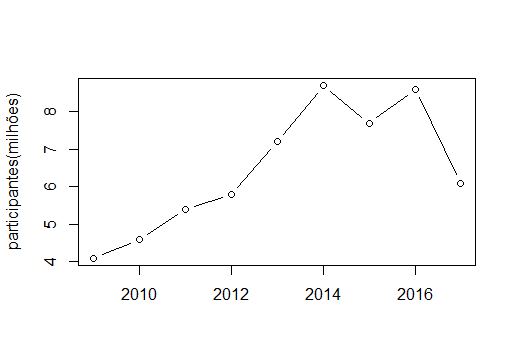
\includegraphics[width=0.5\linewidth]{img/parci}\\
		fonte: INEP(2017)
		\label{fig:parci}
	\end{figure}
    \paragraph{}
    	Entretanto existem críticas a este sistema, Segundo Barretto(2001) os sistemas de avaliação utilizam metodologias e procedimentos altamente sofisticados e se apoiam em um referencial diferente do que habitualmente utilizam os professores, o que pode contribuir para imprimir resistências nas escolas quanto à utilização dos resultados das avaliações.
    	%http://www.ufjf.br/ppge/files/2010/07/Disserta%C3%A7%C3%A3o-flavia-perry.pdf
    \subsection{Enem}
    \paragraph{}
    	De acordo com o MEC para a elaboração  de uma prova  tem-se a necessidade do conhecimento dos parâmetros dos itens. Sendo obtido através de pré-testagens de itens em amostras apropriadas de alunos nas quais estimamos os parâmetros dos itens em uma mesma escala de proficiência. Dessa maneira coloca-se os itens em uma escala de acordo com o nível de proficiência que eles exigem. O conjunto desses itens passa a formam o banco de itens na escala de proficiência desejada e a partir dele pode-se construir um ou mais testes com graus de dificuldade apropriados para atender os objetivos de uma ou mais avaliações. O importante é que as proficiências de alunos submetidos a esses diferentes testes são medidas na mesma escala e, portanto, comparáveis entre si. Da mesma forma, as medidas que se obtêm da proficiência de um aluno submetido a dois testes construídos com itens desse banco serão iguais.
\par
	    O MEC descreve desta forma a pré-testagem, elaboração de itens.
	\subsubsection{Elaboração dos itens}
	\paragraph{}
    	Para que os itens sejam elaborados o Inep recorre a parcerias com instituições de educação superior interessadas em elaborar e revisar itens para a composição das provas do Enem. Estas parcerias têm o objetivo de aumentar a participação da comunidade acadêmica de todo o Brasil nos processos de avaliação educacional, agregando experiência, conhecimento e diversidade.
    \subsubsection{Banco Nacional de itens (BNI)}
    	\paragraph{}
    	Há a necessidade da criação de uma quantidade enorme de itens sendo o Enem é uma avaliação de larga escala, para isso aconteça o INEP gerencia o BNI que consiste em um banco de dados no qual os itens de provas são armazenados de forma segura. Esses itens ficam disponíveis para a construção de provas. A manutenção do BNI depende da entrada constante de itens de qualidade.
    \subsubsection{Pré-teste}
    \paragraph{}
    	Este processo é parte fundamental da calibração dos itens, que consiste na aplicação de um teste contendo itens para uma amostra de alunos com características semelhantes às da população para a qual a prova se destina, os estudantes do ensino médio. Assim esta é a forma empírica de se avaliar a qualidade técnico-pedagógica e psicométrica dos itens. Essa etapa tem como objetivo captar subsídios importantes para aumentar a precisão da prova que será aplicada a milhões de participantes do Enem.
    \subsubsection{Análise depois do Pré-teste}
    \paragraph{}
	    A partir das respostas dos alunos, realiza-se uma série de análises estatísticas e pedagógicas, por exemplo, é avaliado a dificuldade do item, a discriminação e a possibilidade de acerto ao acaso. Depois dessas análises, as questões que atendem aos critérios ficam disponíveis para a montagem das provas, e as demais questões são descartadas ou encaminhadas para reformulação. o enem utilizam o método denominado Expected a Posteriori (EAP).\\
	    \textbf{Questão adequada} - Encaminhada ao Banco Nacional de Itens e utilizada para a elaboração das provas.\\
	    \textbf{Questão inadequada} - Retorna para reformulação ou descarte.\\
	\subsubsection{Elaboração das provas}
	\paragraph{}
    	Durante a seleção dos itens para a composição de uma prova, os índices psicométricos obtidos a partir do pré-teste são utilizados. Outras características consideradas são: conteúdo abordado, temática e habilidade da matriz de referência.
    \newpage
	\begin{figure}[!h]
		\centering
		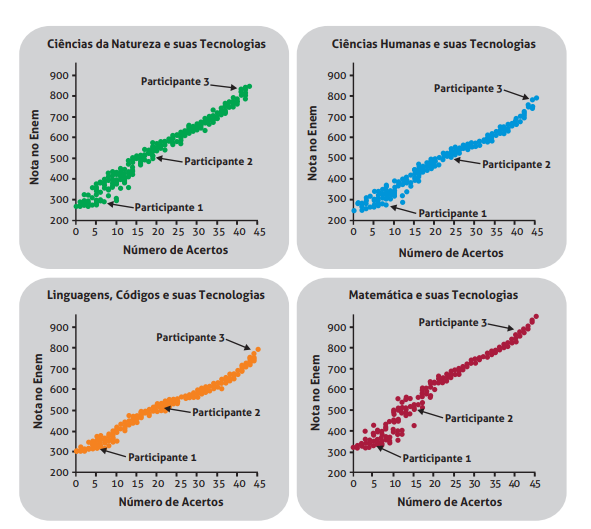
\includegraphics[width=0.4\linewidth]{img/acero}
		\caption{}
		\label{fig:acero}
	\end{figure}
	\paragraph{}
    	Observe que se a nota da TRI fosse exatamente o número de acertos, os pontos nos gráficos estariam alinhados representando uma reta. As variações desses pontos em relação à reta mostram que participantes com o mesmo número de acertos podem ter notas diferentes no Enem. Note, no entanto, que essa variação não é tão grande. O que nos leva a pergunta: Então por que o MEC utiliza a TRI? A resposta está na nota técnica publicada em 2012, onde o MEC diz que: A decisão de implementar no Exame Nacional do Ensino Médio (ENEM) a Teoria de Resposta ao Item (TRI) teve duas finalidades principais:
    \begin{enumerate}
        \item[(1)] permitir a comparabilidade dos resultados entre os anos.
        \item[(2)] permitir a aplicação do Exame várias vezes ao ano. Candidatos poderiam alegar que diferentes provas poderiam ferir o direito de isonomia, mas a tri é igual para todos.
    \end{enumerate}
    	     
	%http://www.sigmees.com.br/files/ARTIGO\_Fernando\_TRI.pdf.
	
	\subsubsection{Coerência pedagógica}
	\paragraph{}
	    O Enem se utiliza desta metodologia que resulta diretamente do modelo logístico de 3 parâmetros devido ao parâmetro de acerto casual.
	\paragraph{}
	    O INEP faz uma analogia, imagine uma competição de corrida com barreiras cuja altura aumenta ao longo do percurso. Imagine, ainda, um atleta que durante os treinos tenha conseguido saltar barreiras de até 80 centímetros. Espera-se que esse atleta, durante a competição, consiga facilmente as barreiras com altura menor que 80 centímetros e tenha dificuldade para saltar barreiras com altura superior. Da mesma forma, espera-se que um participante apresente, coerência pedagógica em suas respostas. saltar durante a prova. Explicando de outra forma se um participante tem um padrão incoerente de respostas este participante terá uma nota menor que que um participante que teve um padrão mais coerente considerando que ambos tiveram a mesma quantidade de acertos.
	
	\begin{figure}[!h]
		\centering
		\caption{padrão coerente}
		\fbox{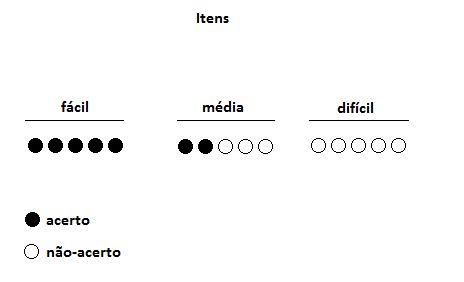
\includegraphics[width=0.5\linewidth]{img/coerente}}\\
		fonte: Autor
		\label{fig:coerente}
	\end{figure}
	\paragraph{}
	    Este padrão é mais corrente, pois o indivíduo acertou os itens fáceis e errou os mais difíceis.
	\begin{figure}[!h]
		\centering
		\caption{padrão incoerente}
		\fbox{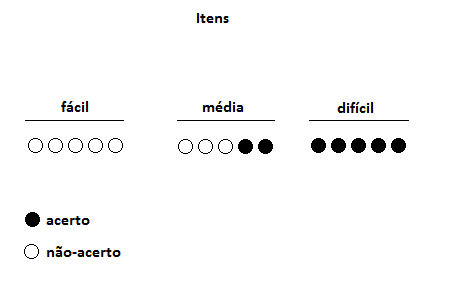
\includegraphics[width=0.5\linewidth]{img/incoerente}}\\
		fonte: Autor
		\label{fig:incoerente}
	\end{figure}
	\paragraph{}
	    Porém, os casos mais comuns Segundo os da Figura(\ref{fig:coerenciax}) no qual o indivíduo responde corretamente itens acerta itens difíceis ocasionalmente e erra itens fáceis ocasionalmente.
	\begin{figure}[!h]
		\centering
		\caption{padrão mais provável}
		\fbox{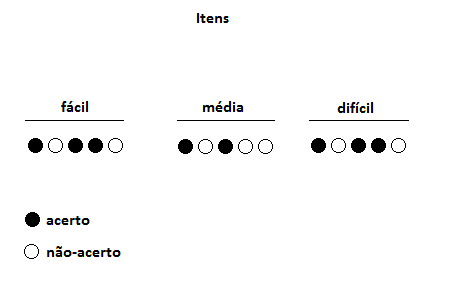
\includegraphics[width=0.5\linewidth]{img/coerenciax}}\\
		fonte: Autor
		\label{fig:coerenciax}
	\end{figure}
	\paragraph{}
	    Entretanto a TRI ao detectar um padrão incoerente como na figura  \ref{fig:incoerente} pode fazer uma analise, julga-se que o individuo que responde corretamente os itens difíceis e responde de forma errada os itens fáceis terá uma nota menor.

	%secao - conclusao
	     \section{CONCLUSÃO}
    \par
    	Com adoção da TRI pelo ENEM, a TRI ganhou notoriedade no cenário acadêmico. Com o avanço computacional e a utilização da TRI em avaliações nacionais e internacionais esta tende a ganha notoriedade no campo acadêmico e educacional.
	\par
    	A TRI tem uma complexidade matemática que não é entendia por todos. Então para que esta metologia seja usada pelas escolas para uma avaliação qualitativa, é necessário grande empenho dos gestores, para qualificação de seus professores.
    \par
	    Apesar dos avanços da área computacional os softwares para TRI ainda não cobrem todos os modelos da TRI, tendo o pesquisador que criar seus próprios programas para estimação das habilidades e parâmetros dos itens. ATRI entrou no Brasil com o objetivo de aprimorar as avaliações educacionais, e considerando a sua aplicação atual no ENEM, não é de se admirar que a maior parte das aplicações tem sido realizada na área de avaliação educacional.
\newpage
	\pagestyle{nohead}
	\renewcommand{\refname}{\hfill REFERÊNCIAS \hfill}
	
	
	\setcounter{section}{7}
	\addcontentsline{toc}{section}{\thesection \hspace{0.3cm} REFERÊNCIAS}
	\medskip
	%\bibliographystyle{abnt-alf}%Used BibTeX style is unsrt
    %\bibliography{bibliografia}
    
    \printbibliography
    % ler https://repositorio.ufsc.br/bitstream/handle/123456789/95506/299657.pdf
	\newpage
   %anexo A
       	\section{ANEXO A - SCRIPIT em R}
\begin{verbatim}
#quantidades
itens <- 20
alunos <- 20
teste <- 50

ais <- runif(itens,1,2)
bis <- rnorm(itens,0,1)
cis <- rnorm(itens,0.2,0.075)

prob <- function(D,hab,a,b,c){
  retrurn <- c + (1 - c)/(1 + exp(-D*a*(hab - b)))
}

habilidades <- rnorm(alunos,0,1)

quant = itens * alunos
for(k in 1:teste){
  x <- matrix(data = rep(1,quant),ncol=itens,nrow=alunos)
  for(i in 1:itens){
    for(j in 1:alunos){
      ran = runif(1)
      ii = (i - 1)*alunos + j
      if(ran < prob(1.7,habilidades[j],ais[i],bis[i],cis[i])){
        x[ii] = 0
      }else{
        x[ii] = 1
      }
    }
  }
  m_s <- paste("matrix",toString(k),".csv",sep="")
  write.csv(x, m_s ,row.names = FALSE)
}

ais_source <- "ais.csv"
bis_source <- "bis.csv"
cis_source <- "cis.csv"
hab_source <- "habilidades.csv"

write.table(ais,ais_source, row.names = FALSE, col.names=FALSE)
write.table(bis,bis_source, row.names = FALSE, col.names=FALSE)
write.table(cis,cis_source, row.names = FALSE, col.names=FALSE)
write.table(habilidades,hab_source, row.names = FALSE, col.names=FALSE)


\end{verbatim}

\end{document}